\documentclass[12pt]{article}
\usepackage{amsmath, amssymb,amsthm,enumerate,bm}
\usepackage{hyperref}
\usepackage{cite}
\usepackage{listings}
\usepackage{pdfpages}

\usepackage[a4paper,bindingoffset=0.2in,%
left=0.8in,right=0.8in,top=1in,bottom=1in,%
footskip=.25in]{geometry}

\DeclareMathOperator*{\argmin}{argmin}
\newcommand{\ttt}[1]{\textbf{#1}}
\newcommand{\la}{\langle}
\newcommand{\ra}{\rangle}
\newcommand{\ip}[4]{\langle \textbf{#1}_{#2} , \textbf{#3}_{#4} \rangle}

\title{Advanced Methods Homework 2}
\date{\today}
\author{Bohao Tang}

\begin{document}
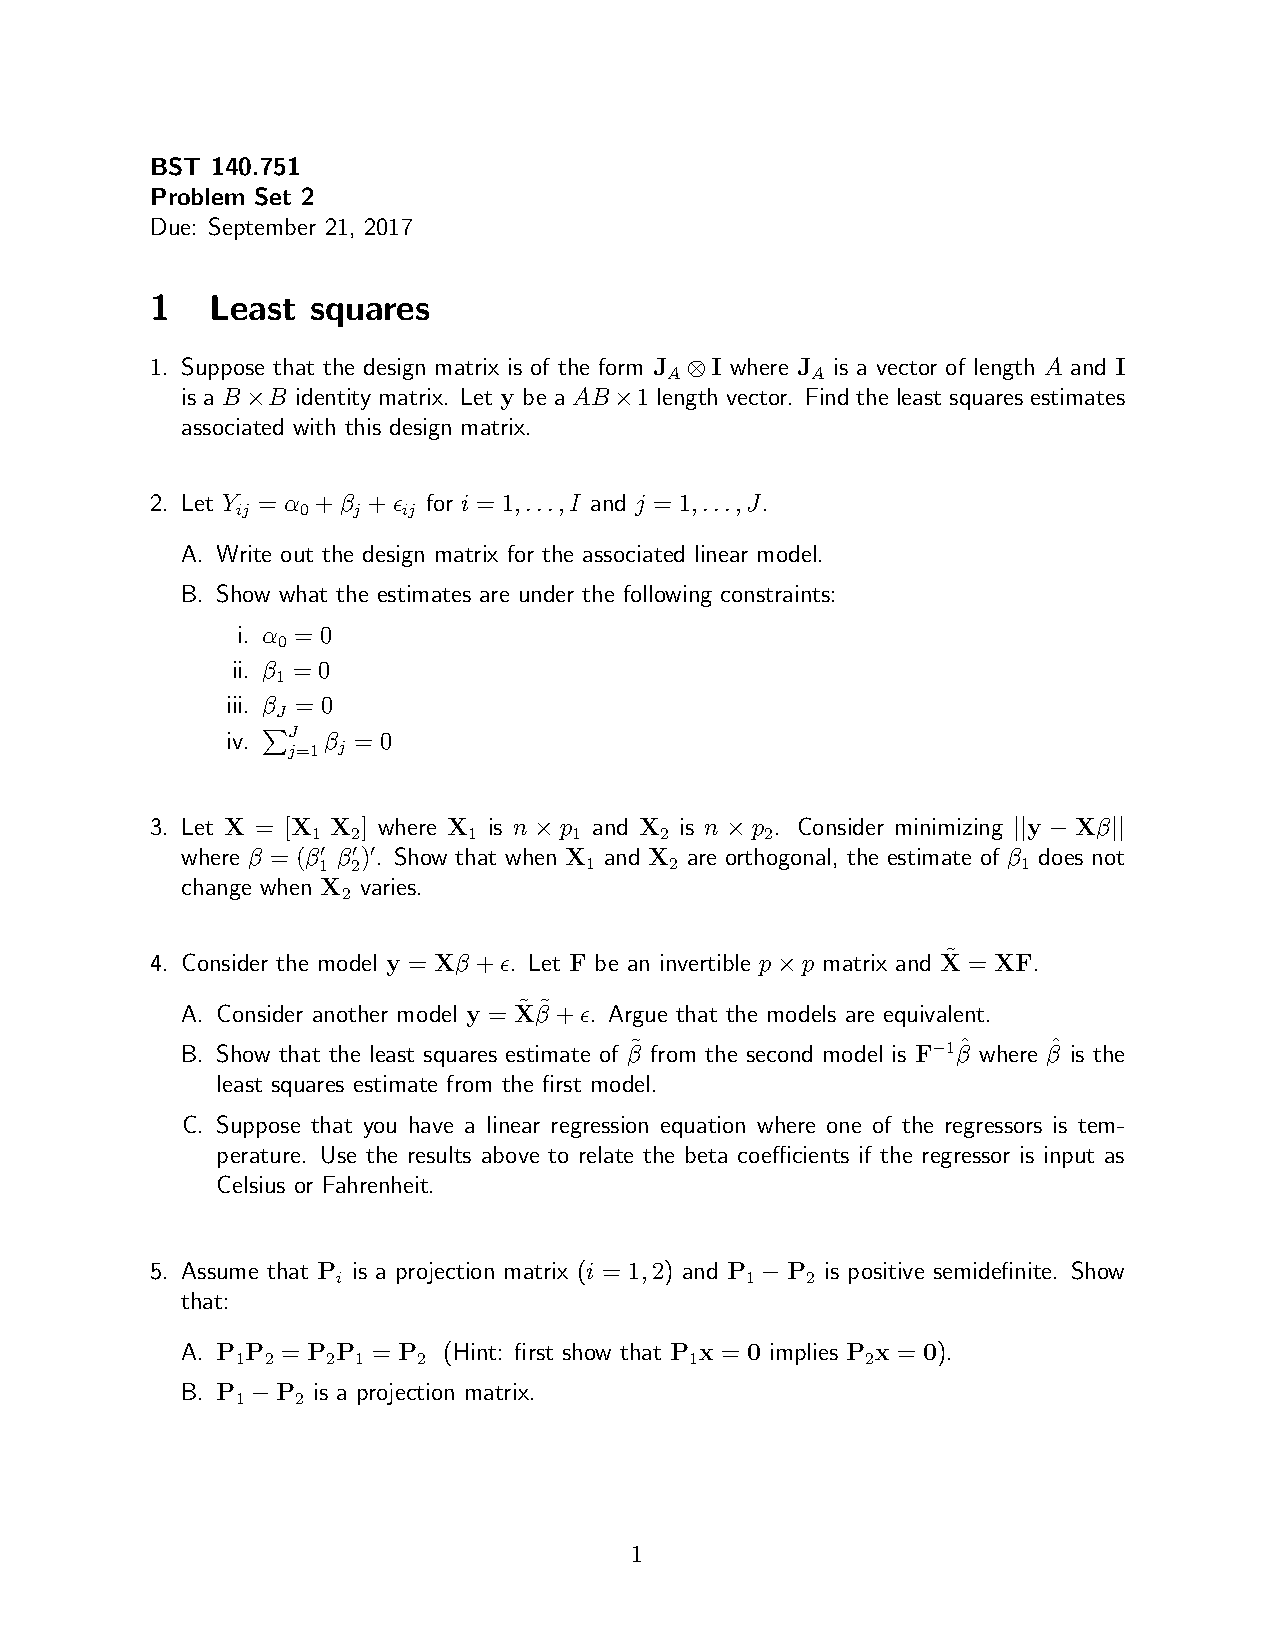
\includepdf[pages=-]{HW2}

\maketitle

\section{Least Squares}
\begin{enumerate}
    \item
    $\ttt{J}_A \otimes \ttt{I}$ is like 
    $\begin{pmatrix}
        \ttt{I} & \ttt{I} & \ttt{I} & \cdots & \ttt{I}
    \end{pmatrix}^\top$.
    Suppose the model is $\ttt{y} = (\ttt{J}_A \otimes \ttt{I})\ \beta + \bm{\epsilon}$. 
    Then we have the estimation $\hat{\beta}$ is $((\ttt{J}_A\otimes\ttt{I})^\top \ttt{J}_A \otimes \ttt{I})^{-1} (\ttt{J}_A \otimes \ttt{I})^\top \ \ttt{y}$. And it is:
    \begin{eqnarray}
        \hat{\beta} &=& \left( \begin{pmatrix} \ttt{I} & \ttt{I} & \cdots & \ttt{I} \end{pmatrix} \begin{pmatrix} \ttt{I} \\ \ttt{I} \\ \vdots \\ \ttt{I} \end{pmatrix} \right)^{-1} \begin{pmatrix} \ttt{I} & \ttt{I} & \cdots & \ttt{I} \end{pmatrix} \ttt{y} \\
                    &=& \frac{1}{A} \ttt{I}\ \sum_{j=1}^{A} \ttt{y}_i = \sum_{j=1}^{A} \ttt{y}_i / A
    \end{eqnarray}
    Where $\ttt{y}_i$ is vectors of length $B$ and $\ttt{y} = \begin{pmatrix}
                                                                    \ttt{y}_1^\top & \ttt{y}_2^\top & \ttt{y}_3^\top & \cdots & \ttt{y}_A^\top
                                                              \end{pmatrix}^\top$
    
    \item
    \begin{enumerate}[A.]
        \item
        $$
        \begin{pmatrix}
            Y_{11}\\
            Y_{12}\\
            Y_{13}\\
            \vdots\\
            Y_{1J}\\
            Y_{21}\\
            Y_{22}\\
            \vdots\\
            Y_{2J}\\
            \vdots\\
            Y_{IJ}\\
        \end{pmatrix} = 
        \begin{pmatrix}
            1 & 1 \\
            1 &  & 1 \\
            1 &  &  & 1 \\
            \vdots &  &  &  & \ddots \\
            1 &  &  &  &  & 1 \\
            1 & 1 \\
            1 &  & 1 \\
            1 &  &  & 1 \\
            \vdots &  &  &  & \ddots \\
            1 &  &  &  &  & 1 \\
            \vdots & \vdots & \vdots & \vdots & \vdots & \vdots \\
            1 & 1 \\
            1 &  & 1 \\
            1 &  &  & 1 \\
            \vdots &  &  &  & \ddots \\
            1 &  &  &  &  & 1 \\
        \end{pmatrix}
        \begin{pmatrix}
            \alpha_0 \\
            \beta_1 \\
            \beta_2 \\
            \vdots \\
            \beta_J\\
        \end{pmatrix} 
        + \bm{\epsilon}
        = \begin{bmatrix}
            \ttt{J}_{IJ} & \ttt{J}_I \otimes \ttt{I}_J
        \end{bmatrix}
        \begin{pmatrix}
            \alpha_0 \\
            \bm{\beta}
        \end{pmatrix} + \bm{\epsilon}
        $$
        So the design matrix is $\begin{bmatrix} \ttt{J}_{IJ} & \ttt{J}_I \otimes \ttt{I}_J \end{bmatrix}$, where $\ttt{I}_J$ is the $J \times J$ identity matrix.
        \item
        \begin{enumerate}[i.]
            \item
            Then the design matrix is $\ttt{J}_I \otimes \ttt{I}_J$, denote $\ttt{Y}_i = \begin{bmatrix} Y_{i1} & Y_{i2} & \cdots & Y_{iJ} \end{bmatrix}^\top$.
            According to question one, we have that $\hat{\beta} = \sum_{j=1}^{I} \ttt{Y}_i / I$.

            \item
            Then the design matrix is $D = \begin{bmatrix} \ttt{J}_{IJ} & \ttt{J}_I \otimes \ttt{L} \end{bmatrix}$, where $\ttt{L} = \begin{pmatrix} \ttt{0} \\ \ttt{I}_{J-1}\end{pmatrix}$.
            So the estimation is (denote $\ttt{Y}_{-1,i} = (Y_{i2},Y_{i3},\cdots,Y_{iJ})^\top$):
            \begin{eqnarray}
                \widehat{(\alpha_0,\beta_2,\cdots,\beta_J)^\top} &=& (D^\top D)^{-1} D^\top \ttt{Y} \\
                                                                 &=& \frac{1}{I} \begin{pmatrix}
                                                                                    J & \ttt{J}_{J-1}^\top \\
                                                                                    \ttt{J}_{J-1} & \ttt{I}_{J-1}
                                                                                 \end{pmatrix}^{-1} \begin{pmatrix} \sum_{i,j}^I Y_{ij} \\ \sum_{i=1}^{I} \ttt{Y}_{-1,i}\end{pmatrix} \\
                                                                 &=& \frac{1}{I} \begin{pmatrix}
                                                                    1 & -\ttt{J}_{J-1}^\top \\
                                                                    -\ttt{J}_{J-1} & \ttt{I}_{J-1} + \ttt{J}_{J-1}\ttt{J}_{J-1}^\top
                                                                 \end{pmatrix} \begin{pmatrix} \sum_{i,j}^I Y_{ij} \\ \sum_{i=1}^{I} \ttt{Y}_{-1,i}\end{pmatrix} \\
                                                                 &=& \begin{pmatrix} \sum_{i=1}^{I} Y_{i1} / I \\ (\sum_{i=1}^{I} \ttt{Y}_{-1,i} - \sum_{i=1}^{I} Y_{i1} \ttt{J}_{J-1}) / I\end{pmatrix}
            \end{eqnarray}

            \item
            Then the design matrix is $D = \begin{bmatrix} \ttt{J}_{IJ} & \ttt{J}_I \otimes \ttt{L}_2 \end{bmatrix}$, where $\ttt{L}_2 = \begin{pmatrix} \ttt{I}_{J-1} \\ \ttt{0}\end{pmatrix}$.
            So the estimation is (denote $\ttt{Y}_{-J,i} = (Y_{i1},Y_{i2},\cdots,Y_{i,J-1})^\top$):
            \begin{eqnarray}
                \widehat{(\alpha_0,\beta_1,\cdots,\beta_{J-1})^\top} &=& (D^\top D)^{-1} D^\top \ttt{Y} \\
                                                                 &=& \frac{1}{I} \begin{pmatrix}
                                                                                    J & \ttt{J}_{J-1}^\top \\
                                                                                    \ttt{J}_{J-1} & \ttt{I}_{J-1}
                                                                                 \end{pmatrix}^{-1} \begin{pmatrix} \sum_{i,j}^I Y_{ij} \\ \sum_{i=1}^{I} \ttt{Y}_{-J,i}\end{pmatrix} \\
                                                                 &=& \frac{1}{I} \begin{pmatrix}
                                                                    1 & -\ttt{J}_{J-1}^\top \\
                                                                    -\ttt{J}_{J-1} & \ttt{I}_{J-1} + \ttt{J}_{J-1}\ttt{J}_{J-1}^\top
                                                                 \end{pmatrix} \begin{pmatrix} \sum_{i,j}^I Y_{ij} \\ \sum_{i=1}^{I} \ttt{Y}_{-J,i}\end{pmatrix} \\
                                                                 &=& \begin{pmatrix} \sum_{i=1}^{I} Y_{iJ} / I \\ (\sum_{i=1}^{I} \ttt{Y}_{-J,i} - \sum_{i=1}^{I} Y_{iJ} \ttt{J}_{J-1}) / I\end{pmatrix}
            \end{eqnarray}

            \item
            We replace $\beta_J$ by $\sum_{i=1}^{J-1} -\beta_i$, then the design matrix $D = \begin{bmatrix} \ttt{J}_{IJ} & \ttt{J}_I \otimes \ttt{L}_3 \end{bmatrix}$, where $\ttt{L}_3 = \begin{pmatrix} \ttt{I}_{J-1} \\ \ttt{J}^\top_{J-1} \end{pmatrix}$.
            So the estimation is:
                \begin{eqnarray}
                    & &\widehat{(\alpha_0,\beta_1,\cdots,\beta_{J-1})}^\top = (D^\top D)^{-1} D^\top \ttt{Y} \\
                                                                     &=& \frac{1}{I} \begin{pmatrix}
                                                                                        J & 0 \\
                                                                                        0 & \ttt{I}_{J-1} + \ttt{J}_{J-1}\ttt{J}_{J-1}^\top
                                                                                     \end{pmatrix}^{-1} \begin{pmatrix} \sum_{i,j}^I Y_{ij} \\ \sum_{i=1}^{I} (\ttt{Y}_{-J,i} - Y_{iJ} \ttt{J}_{J-1})\end{pmatrix} \\
                                                                     &=& \frac{1}{I} \begin{pmatrix}
                                                                        J^{-1} & 0 \\
                                                                        0 & \ttt{I}_{J-1} - \frac{1}{J}\ttt{J}_{J-1}\ttt{J}_{J-1}^\top
                                                                     \end{pmatrix} \begin{pmatrix} \sum_{i,j}^I Y_{ij} \\ \sum_{i=1}^{I} (\ttt{Y}_{-J,i} - Y_{iJ} \ttt{J}_{J-1})\end{pmatrix} \\
                                                                     &=& \begin{pmatrix} \sum_{i,j} Y_{ij} / (IJ) \\ \sum_{i=1}^{I} \ttt{Y}_{-J,i} / I - \sum_{i,j} Y_{ij} \ttt{J}_{J-1} / (IJ)\end{pmatrix}
                \end{eqnarray}
        \end{enumerate}
    \end{enumerate}
    
    \item 
    \begin{proof}
        In the slide of Lecture 5, we get that $\hat{\beta}_1 = (\ttt{X}_1^\top \ttt{X}_1)^{-1} \ttt{X}_1^\top (\ttt{y} - \ttt{X}_2 \hat{\beta}_2)$. 
        And $\hat{\beta}_2$ is $(\ttt{U}^\top \ttt{U})^{-1} \ttt{U}^\top \ttt{V} \ttt{y}$, where $\ttt{U} = (\ttt{I} - \ttt{X}_1(\ttt{X}_1^\top \ttt{X}_1)^{-1} \ttt{X}_1^\top) \ttt{X}_2$, $\ttt{V} = \ttt{I} - \ttt{X}_1(\ttt{X}_1^\top \ttt{X}_1)^{-1} \ttt{X}_1^\top$.

        If $\ttt{X}_1, \ttt{X}_2$ are orthogonal, then $\ttt{X}_1^\top \ttt{X}_2 = \ttt{0}; \ttt{X}_2^\top \ttt{X}_1 = \ttt{0}$.
        Therefore, $\ttt{U} = \ttt{X}_2$ and $\ttt{U}^\top \ttt{V} = \ttt{X}_2$, so $\hat{\beta}_2 = (\ttt{X}_2^\top \ttt{X}_2)^{-1} \ttt{X}_2 \ttt{y}$, and then $\hat{\beta}_1 = (\ttt{X}_1^\top \ttt{X}_1)^{-1} \ttt{X}_1^\top \ttt{y}$.
        So $\hat{\beta}_1$ is not depend on $\ttt{X}_2$ and $\hat{\beta}_2$ is not depend on $\ttt{X}_1$. 
    \end{proof}
    
    \item
    \begin{enumerate}[A.]
        \item
        The projection matrix in new model is:
        $$H = \tilde{\ttt{X}}(\tilde{\ttt{X}}^\top \tilde{\ttt{X}})^{-1}\tilde{\ttt{X}}^\top = \ttt{X}\ttt{F}(\ttt{F}^\top \ttt{X}^\top \ttt{X} \ttt{F})^{-1} \ttt{F}^\top \ttt{X}^\top = \ttt{X}(\ttt{X}^\top \ttt{X})^{-1}\ttt{X}^\top$$
        which is the same with it of design matrix $\ttt{X}$. Therefore, the two models are equivalent in the sense of the projection procedures are the same. (which means the fitted values $\hat{\ttt{y}}$ are the same, and along with result in B., if you get an estimation of the slope of one model, you can simutaneously get the other by a linear transform)
        \item
        \begin{proof}
            $$\hat{\tilde{\beta}} = (\tilde{\ttt{X}}^\top \tilde{\ttt{X}})^{-1}\tilde{\ttt{X}}^\top \ttt{y} = (\ttt{F}^\top \ttt{X}^\top \ttt{X} \ttt{F})^{-1} \ttt{F}^\top \ttt{X}^\top \ttt{y} = \ttt{F}^{-1}(\ttt{X}^\top \ttt{X})^{-1}\ttt{X}^\top \ttt{y} = \ttt{F}^{-1} \hat{\beta}$$    
        \end{proof}
        \item
        Without loss of generality, we can suppose the first regressor is temperature. First, we have the transform formula:
        $$T_{( ^\circ F)} = T_{(^\circ C)} \times \frac{9}{5} + 32$$
        Suppose $\ttt{C}$ is the design matrix with temperature in Celsius ($\ttt{T}_C$) and $\ttt{F}$ is the design matrix with temperature in Fahrenheit ($\ttt{T}_F$). 
        Then denote $(\alpha^C, \beta^C_1, \beta^C_2, \cdots, \beta^C_p)^\top$ are the parameters of temperature in Celsius. $(\alpha^F, \beta^F_1, \beta^F_2, \cdots, \beta^F_p)^\top$ are the parameters of temperature in Fahrenheit.
        We have two models:
        $$ \ttt{y} = \begin{bmatrix} \ttt{J}_n&\ttt{T}_C&\cdots \end{bmatrix} \begin{pmatrix} \alpha^C\\ \beta^C_1\\ \beta^C_2\\ \vdots\\ \beta^C_p \end{pmatrix} + \bm{\epsilon}_1$$
        and 
        \begin{eqnarray}
            \ttt{y} &=& \begin{bmatrix} \ttt{J}_n&\ttt{T}_F&\cdots \end{bmatrix} \begin{pmatrix} \alpha^F\\ \beta^F_1\\ \beta^F_2\\ \vdots\\ \beta^F_p \end{pmatrix} + \bm{\epsilon}_2 \\
                    &=& \begin{bmatrix} \ttt{J}_n & \frac{9}{5}\ttt{T}_C + 32 & \cdots \end{bmatrix} \begin{pmatrix} \alpha^F\\ \beta^F_1\\ \beta^F_2\\ \vdots\\ \beta^F_p \end{pmatrix} + \bm{\epsilon}_2 \\
                    &=& \begin{bmatrix} \ttt{J}_n&\ttt{T}_C&\cdots \end{bmatrix} \begin{pmatrix} \alpha^F + 32 \beta^F_1 \\ \frac{9}{5} \beta^F_1\\ \beta^F_2\\ \vdots\\ \beta^F_p \end{pmatrix} + \bm{\epsilon}_2
        \end{eqnarray}
        So we have that $\hat{\beta}^C_1 = \frac{9}{5} \hat{\beta}^F_1$ and $\hat{\beta}^C_i = \hat{\beta}^F_i$, for all $i > 1$.
    \end{enumerate}

    \item
    \begin{enumerate}[A.]
        \item 
        \begin{proof}
            First, since $P_i$ are projection matrix, then they are symmetric and idempotent. $\forall$ vecotr $\ttt{y}$, $\ttt{y}^\top \ttt{P}_i \ttt{y} = \ttt{y}^\top \ttt{P}_i \ttt{P}_i \ttt{y} = \ttt{y}^\top \ttt{P}_i^\top \ttt{P}_i \ttt{y} = ||\ttt{P}_i \ttt{y}||^2 \ge 0$. So $\ttt{P}_i$ are positive semidefinite.
            For every $\ttt{y}$, we have $\ttt{P}_1 (\ttt{I} - \ttt{P}_1) \ttt{y} = 0$, and $\ttt{P}_1 - \ttt{P}_2, \ttt{P}_i$ are positive semidefinite. Therefore we have:
            $$0 \le [(\ttt{I} - \ttt{P}_1)\ttt{y}]^\top (\ttt{P}_1 - \ttt{P}_2) [(\ttt{I} - \ttt{P}_1)\ttt{y}] = - [(\ttt{I} - \ttt{P}_1)\ttt{y}]^\top \ttt{P}_2 [(\ttt{I} - \ttt{P}_1)\ttt{y}] \le 0$$
            So for every $\ttt{y}$, we have $\ttt{y}^\top (\ttt{I} - \ttt{P}_1)^\top \ttt{P}_2 (\ttt{I} - \ttt{P}_1) \ttt{y} = 0$, then since $(\ttt{I} - \ttt{P}_1)^\top \ttt{P}_2 (\ttt{I} - \ttt{P}_1)$ is symmetric, we have $(\ttt{I} - \ttt{P}_1)^\top \ttt{P}_2 (\ttt{I} - \ttt{P}_1) = \ttt{0}$.
            
            Because:
            $$(\ttt{I} - \ttt{P}_1)^\top \ttt{P}_2 (\ttt{I} - \ttt{P}_1) = (\ttt{I} - \ttt{P}_1)^\top \ttt{P}_2^\top \ttt{P}_2 (\ttt{I} - \ttt{P}_1) = (\ttt{P}_2 (\ttt{I} - \ttt{P}_1))^\top \ttt{P}_2 (\ttt{I} - \ttt{P}_1) = \ttt{0}$$ 
            We have $\ttt{P}_2 (\ttt{I} - \ttt{P}_1) = \ttt{0}$, which shows $\ttt{P}_2 = \ttt{P}_2 \ttt{P}_1$.
            Meanwhile we have $$\ttt{P}_2 = \ttt{P}_2^\top = (\ttt{P}_2 \ttt{P}_1)^\top = \ttt{P}_1^\top \ttt{P}_2^\top = \ttt{P}_1 \ttt{P}_2$$
            Therefore $\ttt{P}_1 \ttt{P}_2 = \ttt{P}_2 \ttt{P}_1 = \ttt{P}_2$.
        \end{proof}

        \item 
        \begin{proof}
            Use results in A. We have:
            $$(\ttt{P}_1 - \ttt{P}_2)^2 = \ttt{P}_1^2 - \ttt{P}_1\ttt{P}_2 -\ttt{P}_2\ttt{P}_1 + \ttt{P}_2^2 = \ttt{P}_1 + \ttt{P}_2 - \ttt{P}_2 - \ttt{P}_2 = \ttt{P}_1 - \ttt{P}_2$$
            Therefore $\ttt{P}_1 - \ttt{P}_2$ is a projection matrix.
        \end{proof}
    \end{enumerate}

\end{enumerate}

\section{Computing and Analysis}
\includepdf[pages=-]{HW2code}

\end{document}